\chapter{Initial proposal}\label{C:innitial-proposal}
This project was proposed by AlterAid a company which is working on several ways to help in taking care of the health of our elderly, or in general, anyone that is relevant to our lives.

This company is working on two different projects that combine together, the first one is called aaaida which consists of a social network where people can stay alert about its relatives, upload information about its health or watch recommendations from doctors or other professionals. On the other side, and more hardware oriented development, they are creating a Sensor Network called HomeSense that once deployed in a house will be able to collect relevant information from those sensors in the home and allow other people to know if the daily life of the resident's house is going normal, or something is happening.

\section{AlterAid products in depth}\label{S:alteraid-products}
As explained before, AlterAid has two relevant products, aaaida which is the unifying social network that shows or even analyzes the data uploaded there. Then comes HomeSense, a Wireles Healthcare Sensor Platform, which is interesting on terms of sensing and daily life control. HomeSense idea is be able to gather information by using distributed sensors around a house and then upload this information to aaaida.

\subsection{HomeSense}\label{SS:HomeSense-proposal}
HomeSense, is a Wireless Healthcare Sensor Platform created with the aim of control and care taking of the elderly and relatives, actually it uses a Netduino Mini which makes the function of the gateway which controls the sensor network, receiving all the data and uploading to aaaida platform through internet.
\\
In the house the communication is carried on using little sensors capable of fetching data in different situations for example a drawer or a medicine cabinet, it is also possible to install the sensors on doors in order to know if they are opened or closed or in any place where is interesting to acquire information from the environment, house or residents. This sensors make use of nRF24LE1 \gls{SoC} with a low-power RF \gls{ISM} band on 2.4GHz from Nordic Semiconductor.
\\
The communication protocol designed for HomeSense is similar to a mesh network with multi-hop transmissions which normally the nodes try to fetch the gateway because this is on charge of upload the information straight to the internet.

\subsection{Case of use}\label{SS:Case-Of-Use}
Alice is a young teenager whose grandfather, Bob, is ill and she wants to know if all is fine in Bob's home life. Alice will sign up in http://www.aaaida.com, there she will create a bond called Bob. A bond is a entity that represents a person, this entity can be configured with different measures. Then Alice will create 2 measures, the first one will be blood pressure while the other one will be bob's house.
In blood pressure, Bob will use a simple elderly-oriented mobile application in order to upload his blood pressure every day, in this manner Alice can be aware of its health.
Apart from this, Alice will buy a product from AlterAid, called HomeSense, which consists of a set of sensors that must be installed in doors, walls, drawers..., a small centralized system that must be plugged to the power and an application to configure HomeSense.
This application will facilitate the linking between Alice account and Bob's bond, in addition, Alice will be able to setup a internet link to HomeSense using grandfather's Internet or a GSM connection to some mobile phone provider.
Once the system is configured and working, Alice will be able to take care of Bob's home life, for example if he must take a pill at the morning, she can control at least if the medicine cabinet has been opened. Or if all doors are closed if Bob is out of home.

\begin{figure}[H]\begin{center}
 \centering
  \captionsetup{justification=centering}
  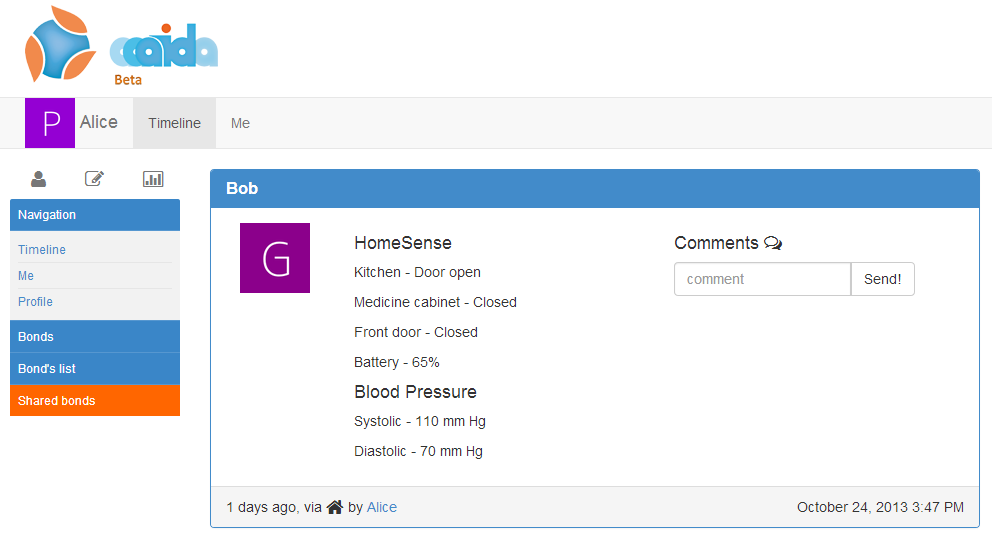
\includegraphics[width=1\textwidth]{pictures/proposal/aaaida-use-case}
  \caption{Case of use representation in aaaida \label{fig:network-architecture}}
\end{center}\end{figure}

\section{AlterNative}\label{S:Proposal-AlterNative}
AlterNative is a language translating tool created by Alex Albal\'{a} and Juan L\'{o}pez. It is capable of translated a compiled (in .NET) binary or library to standard C++ source, basically this program decompiles the the file to be translated, then it sketches how the program works, which are its classes, functions, nodes, etc and then start translating step-by-step all the program, basically it starts writing plain text files with the C++ syntax. After that it links the necessary C++ libraries to work, ones are from boost library, and the other ones are self-written to look like the original C\# classes.
\\
It is interesting to emphasize that the main difference of this translator between the other existing ones is that it tries to generate a code practically identical to the original C\# source code. By doing this, the resulting C++ source is really easy to read for people not used to C++ syntax and language.

\section{Thesis Proposal}\label{S:Proposal-Thesis-Proposal}
After introducing HomeSense and AlterNative is time to explain the thesis proposal itself because it is related to the applications mentioned above. The idea is to take the HomeSense code which runs on closed systems capable of execute a specific .NET framework called Micro Framework, the problem is that the gateway device that runs HomeSense is getting limited in terms of capabilities, performance and expansion for future characteristics.
\\
The idea is to take the gateway code and port it to other devices capable of use minimum GPIO, Interruptions from this ports, the SPI communication protocol and UART because all of them are used in the HomeSense source code. It is important to point that the port must be done on the underlying code which executes Micro Framework code so the original source code should be used without major changes, minor changes such as port renaming and communication module name changing are acceptable because do not alter the original execution flow and design architecture. But not only this should be done on HomeSense, it is interesting to make portable between different hardware platforms any code that runs over Micro Framework.
\\
After accomplishing with this first goal, the second part of the thesis is use AlterNative to translate the IOSharp driver to C++ in order to increase and analyse the performance of IOSharp running on C++ instead of C\#. To accomplish with this some C++ libraries will be need to be written in order to translate IOSharp.